\documentclass[tikz,border=9pt]{standalone}
\usepackage{amsmath,amssymb}
\usetikzlibrary{arrows.meta,positioning,calc}
\begin{document}
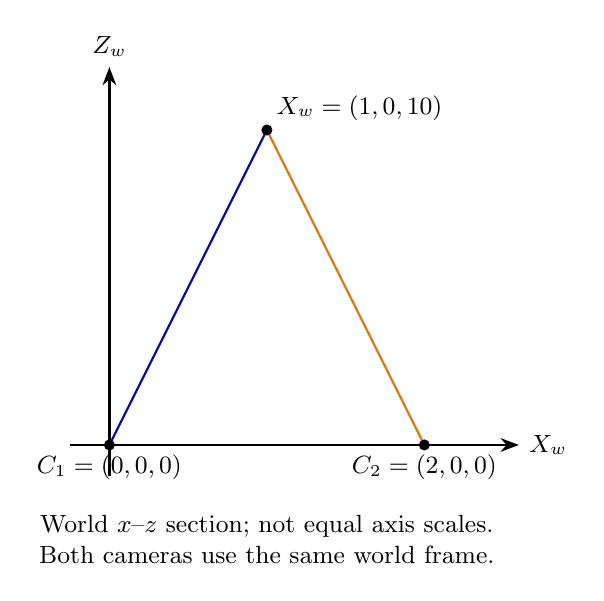
\begin{tikzpicture}[font=\small,arr/.style={-{Stealth},thick},box/.style={draw=blue!55!black,rounded corners,fill=blue!4,align=center,text width=2.9cm,minimum height=1.05cm}]
\coordinate (a) at (0,0);\coordinate (b) at (4,0);\coordinate (p) at (2,4);
\draw[arr] (-.5,0)--(5.2,0) node[right]{$X_w$};\draw[arr] (0,-.4)--(0,4.8) node[above]{$Z_w$};
\draw[thick,blue!70!black] (a)--(p);\draw[thick,orange!90!black] (b)--(p);
\fill (a) circle(2pt) node[below]{$C_1=(0,0,0)$};
\fill (b) circle(2pt) node[below]{$C_2=(2,0,0)$};
\fill (p) circle(2pt) node[above right]{$X_w=(1,0,10)$};
\node[align=center] at (2,-1.2){World $x$--$z$ section; not equal axis scales.\\Both cameras use the same world frame.};
\end{tikzpicture}
\end{document}
